% =============================================================================
%  Machine Learning for Petroleum Engineers Using Python
%  Módulo 7 · Clase 4: Las Máquinas que Ven --- la última clase
%  SLB Ecuador | UDLA
%
%  Compilar: pdflatex -shell-escape presentacion.tex (x2 para refs)
% =============================================================================
\documentclass[aspectratio=169, 11pt]{beamer}

% ── Codificación y lenguaje ──────────────────────────────────────────────────
\usepackage[T1]{fontenc}
\usepackage[utf8]{inputenc}
\usepackage[spanish,es-noshorthands]{babel}

% ── Fuentes ──────────────────────────────────────────────────────────────────
\usepackage{FiraSans}
\usepackage{FiraMono}
\renewcommand{\familydefault}{\sfdefault}

% ── Gráficos y diagramas ────────────────────────────────────────────────────
\usepackage{graphicx}
\usepackage{tikz}
\usetikzlibrary{arrows.meta, positioning, shapes.geometric, calc, fit, decorations.pathreplacing}
\usepackage{fontawesome5}

% ── Código fuente ────────────────────────────────────────────────────────────
\usepackage{minted}
\usepackage{tcolorbox}
\tcbuselibrary{minted, skins, breakable}

% ── Tablas y utilidades ──────────────────────────────────────────────────────
\usepackage{amsmath}
\usepackage{colortbl}
\usepackage{booktabs}
\usepackage{multicol}
\usepackage{hyperref}
\usepackage{calc}

% =============================================================================
%  PALETA DE COLORES (rojo UDLA + variantes)
% =============================================================================
\definecolor{arcaRed}{HTML}{C82B40}
\definecolor{arcaDark}{HTML}{6B1525}
\definecolor{udlaCrimson}{HTML}{A31545}
\definecolor{arcaGray}{HTML}{F5F5F5}
\definecolor{arcaLightGray}{HTML}{EBEBEB}
\definecolor{textDark}{HTML}{2D2D2D}
\definecolor{textMuted}{HTML}{6B7280}
\definecolor{codeGreen}{HTML}{16A34A}
\definecolor{codeBlue}{HTML}{2563EB}
\definecolor{codeOrange}{HTML}{EA580C}
\definecolor{slbBlue}{HTML}{0014DC}
\definecolor{terminalBg}{HTML}{0F172A}
\definecolor{terminalGreen}{HTML}{86EFAC}
\definecolor{terminalMuted}{HTML}{94A3B8}
\definecolor{codeBg}{HTML}{FAFAFA}

% =============================================================================
%  CONFIGURACIÓN DEL TEMA BEAMER
% =============================================================================
\usetheme{default}
\usecolortheme{default}

\setbeamertemplate{navigation symbols}{}
\setbeamertemplate{footline}{}
\setbeamertemplate{headline}{}

\setbeamercolor{normal text}{fg=textDark}
\setbeamercolor{frametitle}{fg=arcaRed, bg=white}
\setbeamercolor{title}{fg=white}
\setbeamercolor{subtitle}{fg=white!85}
\setbeamercolor{author}{fg=white!80}
\setbeamercolor{date}{fg=white!70}
\setbeamercolor{item}{fg=arcaRed}
\setbeamercolor{subitem}{fg=arcaDark}
\setbeamercolor{block title}{fg=white, bg=arcaRed}
\setbeamercolor{block body}{fg=textDark, bg=arcaGray}
\setbeamercolor{block title alerted}{fg=white, bg=codeOrange}
\setbeamercolor{block body alerted}{fg=textDark, bg=arcaGray}
\setbeamercolor{block title example}{fg=white, bg=codeGreen}
\setbeamercolor{block body example}{fg=textDark, bg=arcaGray}
\setbeamercolor{section in toc}{fg=arcaDark}

\setbeamerfont{frametitle}{size=\Large, series=\bfseries}
\setbeamerfont{title}{size=\huge, series=\bfseries}
\setbeamerfont{subtitle}{size=\large}
\setbeamerfont{author}{size=\normalsize}
\setbeamerfont{date}{size=\small}
\setbeamerfont{block title}{size=\normalsize, series=\bfseries}
\setbeamerfont{footnote}{size=\tiny}

\setbeamertemplate{itemize item}{\scriptsize\raise1.5pt\hbox{\color{arcaRed}$\blacktriangleright$}}
\setbeamertemplate{itemize subitem}{\scriptsize\raise1pt\hbox{\color{arcaDark}$\bullet$}}
\setbeamertemplate{enumerate items}[default]
\setbeamercolor{enumerate item}{fg=arcaRed}

% =============================================================================
%  HEADER
% =============================================================================
\setbeamertemplate{headline}{%
  \begin{tikzpicture}[remember picture, overlay]
    \fill[arcaDark] (current page.north west) rectangle
      ([yshift=-0.7cm]current page.north east);
    \node[anchor=west, inner sep=0pt] at
      ([xshift=0.6cm, yshift=-0.35cm]current page.north west)
      {
\includegraphics[height=0.45cm]{../logo_udla_white.png}};
    \node[anchor=east, inner sep=0pt] at
      ([xshift=-0.6cm, yshift=-0.35cm]current page.north east)
      {
\includegraphics[height=0.42cm]{../SLB_white.png}};
  \end{tikzpicture}%
  \vspace{0.7cm}%
}

% =============================================================================
%  FOOTER
% =============================================================================
\setbeamertemplate{footline}{%
  \begin{tikzpicture}[remember picture, overlay]
    \draw[arcaLightGray, line width=0.4pt]
      ([yshift=0.55cm, xshift=0.6cm]current page.south west) --
      ([yshift=0.55cm, xshift=-0.6cm]current page.south east);
    \node[anchor=south, font=\tiny\color{textMuted}] at
      ([yshift=0.15cm]current page.south)
      {Machine Learning for Petroleum Engineers Using Python \(\cdot\) SLB Ecuador};
    \node[anchor=south east, font=\scriptsize\bfseries\color{arcaRed}] at
      ([xshift=-0.6cm, yshift=0.15cm]current page.south east)
      {\insertframenumber};
  \end{tikzpicture}%
}

% =============================================================================
%  FRAMETITLE personalizado con línea roja
% =============================================================================
\setbeamertemplate{frametitle}{%
  \vspace{0.25cm}%
  \usebeamerfont{frametitle}\usebeamercolor[fg]{frametitle}\insertframetitle%
  \par\vspace{2pt}%
  \begin{tikzpicture}
    \fill[arcaRed] (0,0) rectangle (3cm, 1.5pt);
    \fill[arcaLightGray] (3cm,0) rectangle (\textwidth, 0.5pt);
  \end{tikzpicture}%
  \vspace{0.1cm}%
}

% =============================================================================
%  ESTILO DE BLOQUES DE CÓDIGO (minted + tcolorbox)
% =============================================================================
\newtcblisting{pyblock}[1][]{%
  listing engine=minted,
  minted language=python,
  minted style=xcode,
  minted options={
    fontsize=\small,
    linenos=false,
    breaklines=true,
    python3=true
  },
  enhanced,
  colback=codeBg,
  colframe=arcaRed,
  left=8pt,
  right=6pt,
  top=5pt,
  bottom=5pt,
  boxrule=0pt,
  leftrule=3pt,
  arc=3pt,
  listing only,
  title={\hspace{-2pt}\faPython\hspace{5pt}Python},
  fonttitle=\scriptsize\bfseries,
  colbacktitle=arcaRed,
  coltitle=white,
  attach boxed title to top left={xshift=8pt, yshift=-7pt},
  boxed title style={
    arc=2pt, boxrule=0pt,
    top=1.5pt, bottom=1.5pt, left=6pt, right=6pt
  },
  drop fuzzy shadow=black!12,
  #1
}

\newtcblisting{outputblock}[1][]{%
  listing engine=minted,
  minted language=text,
  minted style=bw,
  minted options={
    fontsize=\small,
    breaklines=true,
    formatcom=\color{terminalGreen}
  },
  enhanced,
  colback=terminalBg,
  colframe=terminalBg,
  coltext=terminalGreen,
  left=10pt, right=6pt, top=5pt, bottom=5pt,
  boxrule=0pt,
  arc=3pt,
  listing only,
  title={\hspace{-2pt}\faTerminal\hspace{5pt}Output},
  fonttitle=\scriptsize\bfseries,
  colbacktitle=terminalGreen!85!black,
  coltitle=terminalBg,
  attach boxed title to top left={xshift=8pt, yshift=-7pt},
  boxed title style={
    arc=2pt, boxrule=0pt,
    top=1.5pt, bottom=1.5pt, left=6pt, right=6pt
  },
  #1
}

% =============================================================================
%  SECTION DIVIDERS
% =============================================================================
\newcommand{\sectionframe}[2]{%
  \begingroup
    \setbeamertemplate{headline}{}
    \setbeamertemplate{footline}{}
    \setbeamertemplate{navigation symbols}{}
    \begin{frame}[plain, noframenumbering]
      \begin{tikzpicture}[remember picture, overlay]
        \fill[arcaRed] (current page.south west) rectangle (current page.north east);
        \node[anchor=center, text=white, font=\Huge\bfseries, text width=15cm,
              align=center] at ([yshift=0.5cm]current page.center)
              {\hyphenpenalty=10000\exhyphenpenalty=10000 #1};
        \node[anchor=center, text=white!80, font=\large, text width=10cm,
              align=center] at ([yshift=-0.8cm]current page.center) {#2};
      \end{tikzpicture}
    \end{frame}
  \endgroup
}

% =============================================================================
%  METADATOS
% =============================================================================
\title{Machine Learning for Petroleum Engineers\\Using Python}
\subtitle{Módulo 7 · Clase 4: Las Máquinas que Ven}
\author{Carlos Enrique Mosquera Trujillo}
\date{2026}

% =============================================================================
%  DOCUMENTO
% =============================================================================
% =============================================================================
%  DOCUMENTO
% =============================================================================
\begin{document}
% ── PORTADA ──────────────────────────────────────────────────────────────────
{
\setbeamertemplate{headline}{}
\setbeamertemplate{footline}{}
\begin{frame}[plain, noframenumbering]
  \begin{tikzpicture}[remember picture, overlay]
    \fill[white] (current page.south west) rectangle (current page.north east);
    \fill[arcaRed] (current page.north west) rectangle ([yshift=-0.35cm]current page.north east);
    \fill[arcaDark] (current page.south west) rectangle ([yshift=0.35cm]current page.south east);
    \fill[arcaRed]
      ([xshift=1.1cm, yshift=-0.35cm]current page.north west) rectangle
      ([xshift=1.15cm, yshift=0.35cm]current page.south west);
    \node[anchor=north west, inner sep=0pt] at
      ([xshift=1.8cm, yshift=-1.2cm]current page.north west)
      {
\includegraphics[height=1.6cm]{../logo_udla.png}};
    \node[anchor=north east, inner sep=0pt] at
      ([xshift=-1.5cm, yshift=-1.2cm]current page.north east)
      {
\includegraphics[height=1.5cm]{../SLB.png}};
    \node[anchor=center, text=arcaDark, text width=14.5cm, align=center] at
      ([yshift=0.95cm]current page.center) {
        {\LARGE\bfseries Machine Learning for Petroleum Engineers}\\[8pt]
        {\LARGE\bfseries Using Python}
      };
    \fill[arcaRed]
      ([yshift=-0.35cm, xshift=-3.2cm]current page.center) rectangle
      ([yshift=-0.28cm, xshift=3.2cm]current page.center);
    \node[anchor=center, text=arcaRed, font=\large, text width=13cm, align=center] at
      ([yshift=-1.3cm]current page.center) {
        Módulo 7 · Clase 4 --- la última\\[3pt]
        Las Máquinas que Ven
      };
    \node[anchor=center, text=textMuted, font=\normalsize] at
      ([yshift=-2.5cm]current page.center) {
        {\color{arcaRed}\faUser}\hspace{6pt}Carlos Enrique Mosquera Trujillo
        \hspace{16pt}
        {\color{arcaRed}\faIndustry}\hspace{4pt}SLB Ecuador
      };
  \end{tikzpicture}
\end{frame}
}

\begin{frame}[shrink=5]{Dónde Estamos: la Última Clase}
  \vspace{-2pt}
  {\scriptsize\color{textMuted}
   Cinco partes, y todas suman piezas para \textbf{su entrega del jueves}:}
  \vspace{2pt}
  {\scriptsize\color{textMuted}
  \begin{enumerate}\setlength{\itemsep}{2pt}
    \item \textbf{La solución del reto} --- Fashion-MNIST, corregido como un
          examen.
    \item \textbf{La GPU} --- el paréntesis que vale billones, y el botón que
          les toca.
    \item \textbf{El mapa de la visión} --- las tareas, y en qué se
          diferencian.
    \item \textbf{Cada tarea, con código} --- cuatro modelos, la misma línea.
          Y el \textbf{ojo por código}: Gemini multimodal desde la celda.
    \item \textbf{Los peligros, con nombre} --- la promesa pendiente, pagada.
  \end{enumerate}}
  \vspace{2pt}
  \begin{tcolorbox}[colback=arcaGray, colframe=arcaRed, boxrule=0pt,
    leftrule=3pt, arc=3pt, left=8pt, right=8pt, top=4pt, bottom=4pt]
    {\scriptsize\color{arcaRed}\bfseries LA LLAVE DE LA CLASE}\\[2pt]
    {\scriptsize\color{textMuted}
     Llega por el chat del curso. Va directo a los \textbf{Secrets de Colab}
     (\faKey), con el nombre \texttt{LLAVE\_CLASE}. Nunca pegada en una
     celda --- y al final de la clase la \textbf{revocamos en vivo}. Eso
     también es lección.}
  \end{tcolorbox}
\end{frame}

% ═════════════════════════════════════════════════════════════════════════════
\sectionframe{1 · La Solución del Reto}{Fashion-MNIST, corregido como un examen \\[6pt] \normalsize 0 -- 20 min}
% ═════════════════════════════════════════════════════════════════════════════

\begin{frame}[shrink=8]{La Misma Red, Otro Dato}
  \vspace{-2pt}
  \begin{center}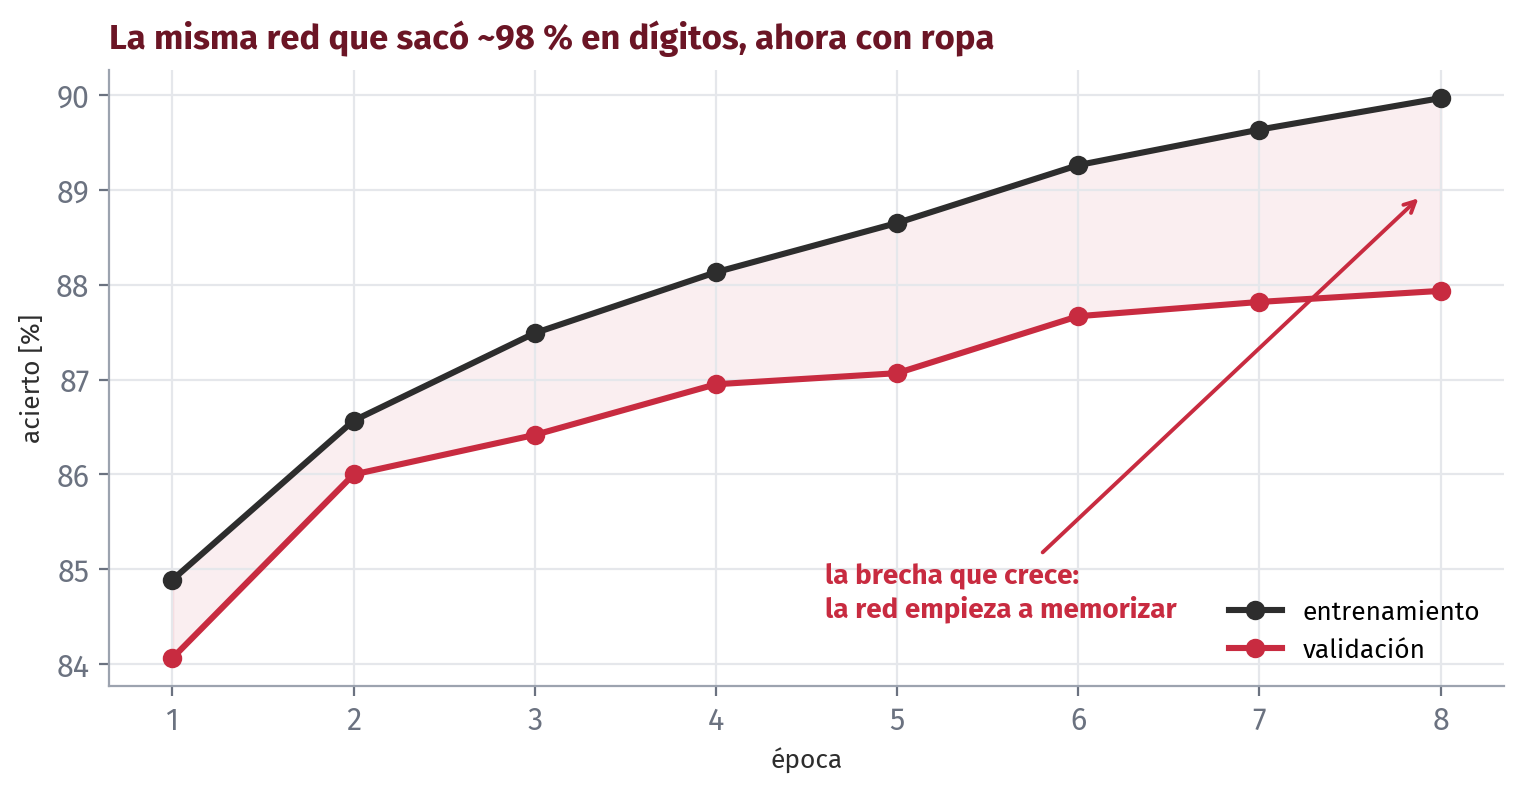
\includegraphics[width=0.86\textwidth, height=0.46\textheight, keepaspectratio]{fig_sol_curvas.png}\end{center}
  \vspace{2pt}
  {\footnotesize\color{textMuted}
   La red que sacó \textbf{~98\,\%} con dígitos, idéntica, da \textbf{~87\,\%}
   con ropa --- y sus curvas se separan: entrenamiento 90, validación 88.
   \emph{(Corrida de referencia; la de ustedes varía en decimales, las
   lecciones no.)}}
\end{frame}

\begin{frame}[shrink=8]{Dónde Se Equivoca}
  \vspace{-2pt}
  \begin{center}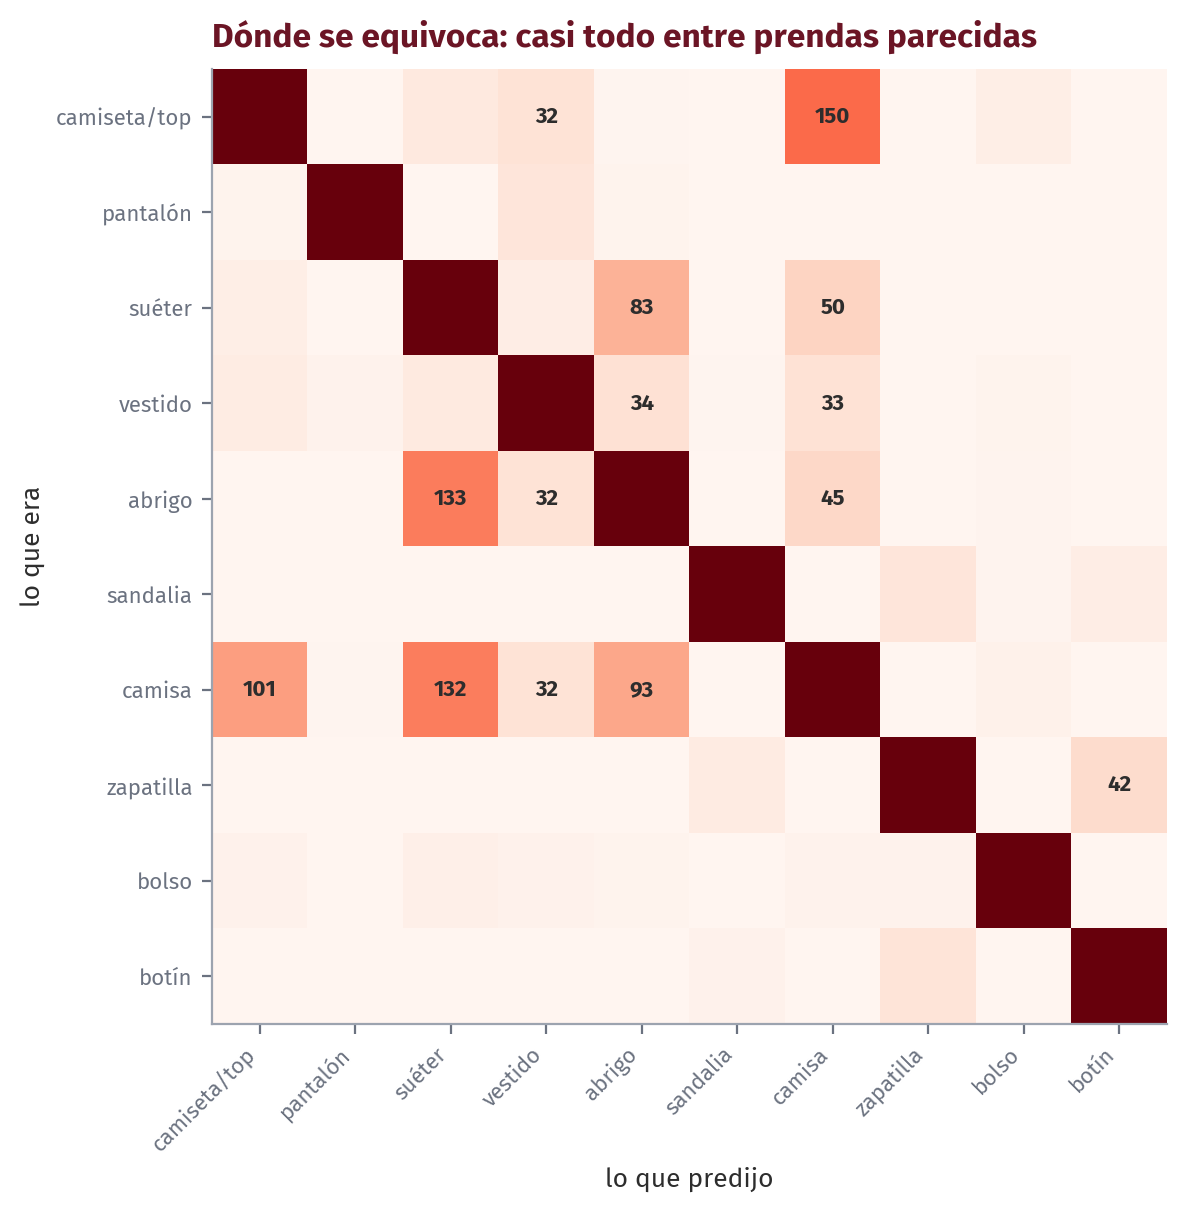
\includegraphics[width=0.60\textwidth, height=0.50\textheight, keepaspectratio]{fig_sol_confusion.png}\end{center}
  \vspace{2pt}
  {\footnotesize\color{textMuted}
   Casi todo el error vive entre \textbf{prendas parecidas}: camiseta que
   cree camisa (150 veces), abrigo que cree suéter (133), camisa que cree
   suéter (132). El pantalón y el bolso casi no fallan.}
\end{frame}

\begin{frame}[shrink=8]{Los Errores, Mirados a la Cara}
  \vspace{-2pt}
  \begin{center}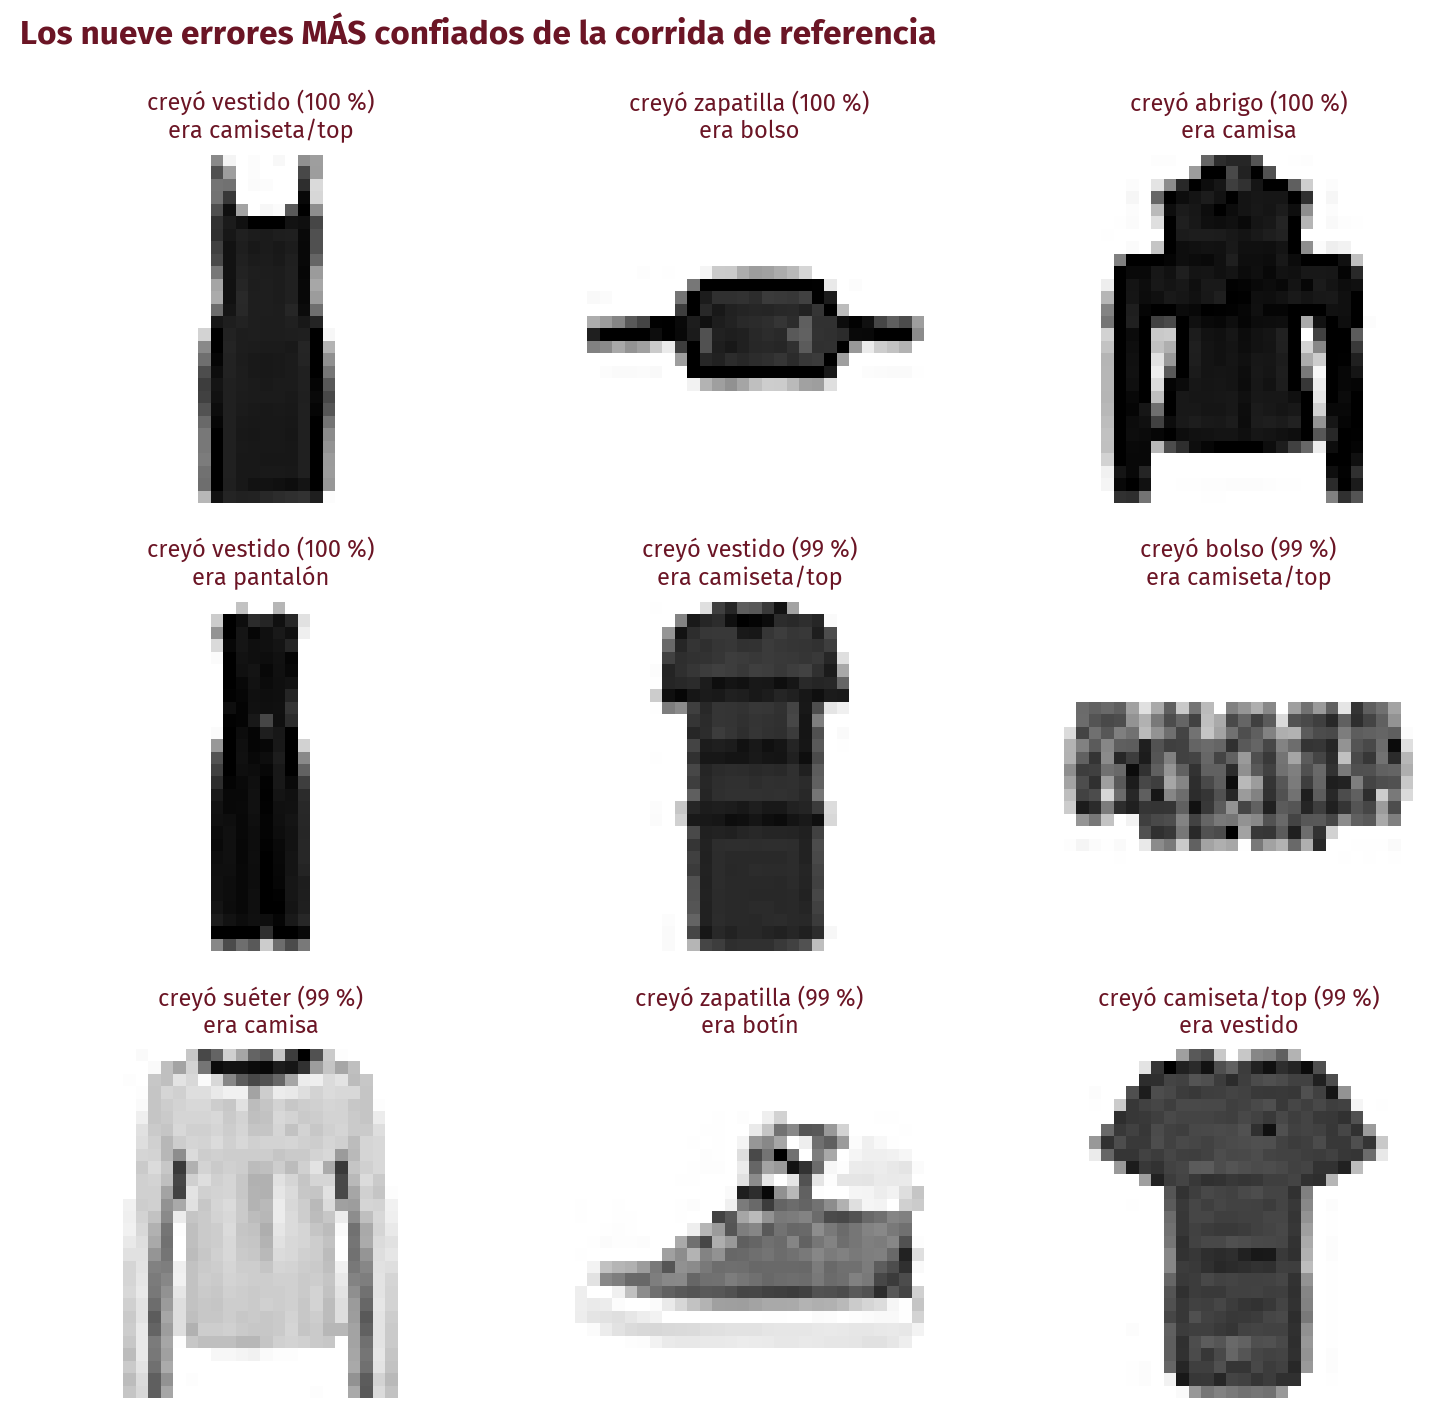
\includegraphics[width=0.54\textwidth, height=0.50\textheight, keepaspectratio]{fig_sol_errores.png}\end{center}
  \vspace{2pt}
  {\footnotesize\color{textMuted}
   Los nueve errores \textbf{más confiados}. Pregunta para la sala: en
   28×28 píxeles, ¿ustedes lo habrían hecho mejor?}
\end{frame}

\begin{frame}[shrink=5]{Las Tres Lecciones de la Solución}
  \vspace{2pt}
  {\footnotesize\color{textMuted}
  \begin{enumerate}\setlength{\itemsep}{6pt}
    \item \textbf{La dificultad vive en el dato, no en la arquitectura.}
          Misma red, mismo entrenamiento: 98 contra 87.
    \item \textbf{Las confusiones son las humanas.} Camiseta$\leftrightarrow$camisa,
          abrigo$\leftrightarrow$suéter --- el modelo falla donde fallaríamos nosotros.
    \item \textbf{El techo no se sube con más épocas} --- eso solo memoriza,
          y lo dicen sus propias curvas.
  \end{enumerate}}
  \vspace{7pt}
  \begin{tcolorbox}[colback=arcaGray, colframe=codeGreen, boxrule=0pt,
    leftrule=4pt, arc=3pt, left=10pt, right=10pt, top=6pt, bottom=6pt]
    {\footnotesize\color{arcaDark}\bfseries
     El techo se sube cambiando de arquitectura: una que entienda que un
     píxel y sus \emph{vecinos} forman bordes y texturas. Esa idea se llama
     \textbf{convolución} --- y es la puerta de todo lo que sigue hoy.}
  \end{tcolorbox}
  \vspace{5pt}
  {\scriptsize\color{arcaDark}\itshape
   Nuestra red Dense miraba 784 píxeles sueltos, sin saber cuáles eran
   vecinos. Una red convolucional aprende \emph{patrones locales} y los
   compone. Es la misma idea de apilar dobleces --- llevada al espacio.}
\end{frame}

% ═════════════════════════════════════════════════════════════════════════════
\sectionframe{2 · El Paréntesis que Vale Billones}{Qué es una GPU, y por qué hay que encenderla \\[6pt] \normalsize 20 -- 30 min}
% ═════════════════════════════════════════════════════════════════════════════

\begin{frame}[shrink=5]{CPU y GPU, Desde Cero}
  \vspace{2pt}
  {\scriptsize\color{textMuted}
   ¿Notaron que entrenar la red \textbf{tardó}? Corrió en la CPU. La
   diferencia, sin jerga:}
  \vspace{2pt}
  \begin{columns}[T]
    \begin{column}{0.47\textwidth}
      \begin{tcolorbox}[colback=arcaGray, colframe=arcaDark, boxrule=0pt,
        leftrule=3pt, arc=3pt, left=8pt, right=8pt, top=4pt, bottom=4pt]
        {\scriptsize\color{arcaDark}\bfseries CPU --- el cirujano}\\[3pt]
        {\scriptsize\color{textMuted}
         Unos pocos núcleos, rapidísimos y versátiles: hacen
         \emph{cualquier} cosa, una tras otra. Perfecta para lógica,
         decisiones, tareas distintas encadenadas.}
      \end{tcolorbox}
    \end{column}
    \begin{column}{0.47\textwidth}
      \begin{tcolorbox}[colback=arcaGray, colframe=codeGreen, boxrule=0pt,
        leftrule=3pt, arc=3pt, left=8pt, right=8pt, top=4pt, bottom=4pt]
        {\scriptsize\color{codeGreen}\bfseries GPU --- la cuadrilla}\\[3pt]
        {\scriptsize\color{textMuted}
         \textbf{Miles} de núcleos pequeños que hacen \emph{la misma
         operación sobre muchos datos a la vez}. Mil obreros, el mismo
         movimiento, al unísono.}
      \end{tcolorbox}
    \end{column}
  \end{columns}
  \vspace{2pt}
  \begin{tcolorbox}[colback=arcaGray, colframe=arcaRed, boxrule=0pt,
    leftrule=4pt, arc=3pt, left=10pt, right=10pt, top=4pt, bottom=4pt]
    {\scriptsize\color{arcaDark}\bfseries
     Una red neuronal es, por dentro, casi pura multiplicación de matrices:
     millones de operaciones idénticas e independientes. Exactamente el
     trabajo de la cuadrilla.}
  \end{tcolorbox}
\end{frame}

\begin{frame}[shrink=5]{De los Videojuegos a 4 Billones de Dólares}
  \vspace{2pt}
  {\scriptsize\color{textMuted}
  \begin{itemize}\setlength{\itemsep}{2pt}
    \item[{\color{arcaRed}\bfseries 1993}]
      Nace \textbf{NVIDIA} para una sola cosa: dibujar videojuegos ---
      millones de píxeles en paralelo. La matemática correcta, sin que
      nadie supiera aún para qué más serviría.
    \item[{\color{arcaRed}\bfseries 2007}]
      \textbf{CUDA}: NVIDIA abre sus tarjetas al cómputo general. Los
      científicos descubren la cuadrilla.
    \item[{\color{arcaRed}\bfseries 2012}]
      El momento bisagra: \textbf{AlexNet}, una red entrenada en \textbf{dos
      GPUs de videojuegos}, arrasa la competencia de reconocimiento de
      imágenes ImageNet. Arranca la era del deep learning.
    \item[{\color{arcaRed}\bfseries 2026}]
      NVIDIA es de las empresas más valiosas del mundo --- del orden de los
      \textbf{4 billones de dólares} --- y la GPU es el recurso estratégico
      de la IA: se compra por decenas de miles, con listas de espera y
      geopolítica de por medio.
  \end{itemize}}
  \vspace{2pt}
  \begin{tcolorbox}[colback=arcaGray, colframe=codeGreen, boxrule=0pt,
    leftrule=4pt, arc=3pt, left=10pt, right=10pt, top=4pt, bottom=4pt]
    {\scriptsize\color{arcaDark}\bfseries
     Y el botón que a ustedes les toca: Colab $\to$ Entorno de ejecución
     $\to$ Cambiar tipo $\to$ \textbf{GPU (T4)} --- gratis.}\\[3pt]
    {\scriptsize\color{textMuted}
     Ojo: al cambiar, \textbf{la sesión se reinicia} --- se vuelven a correr
     las celdas. Háganlo ahora, antes de la parte de visión.}
  \end{tcolorbox}
\end{frame}

% ═════════════════════════════════════════════════════════════════════════════
\sectionframe{3 · El Mapa de la Visión}{Cada tarea es una pregunta distinta \\[6pt] \normalsize 30 -- 40 min}
% ═════════════════════════════════════════════════════════════════════════════

\begin{frame}[shrink=5]{Las Tareas, y la Pregunta que Responde Cada Una}
  \vspace{4pt}
  \begin{center}
  {\footnotesize
  \begin{tabular}{lll}
    \toprule
    \textbf{Tarea} & \textbf{La pregunta} & \textbf{En su mundo} \\
    \midrule
    Clasificación & ¿\emph{qué} es esta imagen? & ¿junta corroída o sana? \\[2pt]
    Detección & ¿\emph{qué} hay, y \emph{dónde}? & cascos y chalecos en cámara \\[2pt]
    Segmentación & ¿\emph{qué píxeles} exactamente? & el área exacta del derrame \\[2pt]
    Pose & ¿en qué \emph{posición}? & ergonomía; persona caída \\[2pt]
    OCR / lectura & ¿qué \emph{dice}? & medidores, placas, documentos \\[2pt]
    Multimodal & \emph{cualquier} pregunta & «describe esta foto» \\
    \bottomrule
  \end{tabular}}
  \end{center}
  \vspace{8pt}
  {\footnotesize\color{arcaDark}\bfseries
   Saber cuál pedir es el 80\,\% del trabajo --- es la versión visual de
   «especificar bien».}
  \vspace{5pt}

  {\footnotesize\color{textMuted}
   Las cuatro primeras las corremos ahora, \textbf{con código, una por una}.
   Las dos últimas, con el ojo por código de la parte 5.}
\end{frame}

% ═════════════════════════════════════════════════════════════════════════════
\sectionframe{4 · Cada Tarea, con Código}{Cuatro modelos, la misma línea --- y el ojo por código \\[6pt] \normalsize 40 -- 95 min}
% ═════════════════════════════════════════════════════════════════════════════

\begin{frame}[shrink=8]{La Lámina Completa: una Foto, Cuatro Preguntas}
  \vspace{-2pt}
  \begin{center}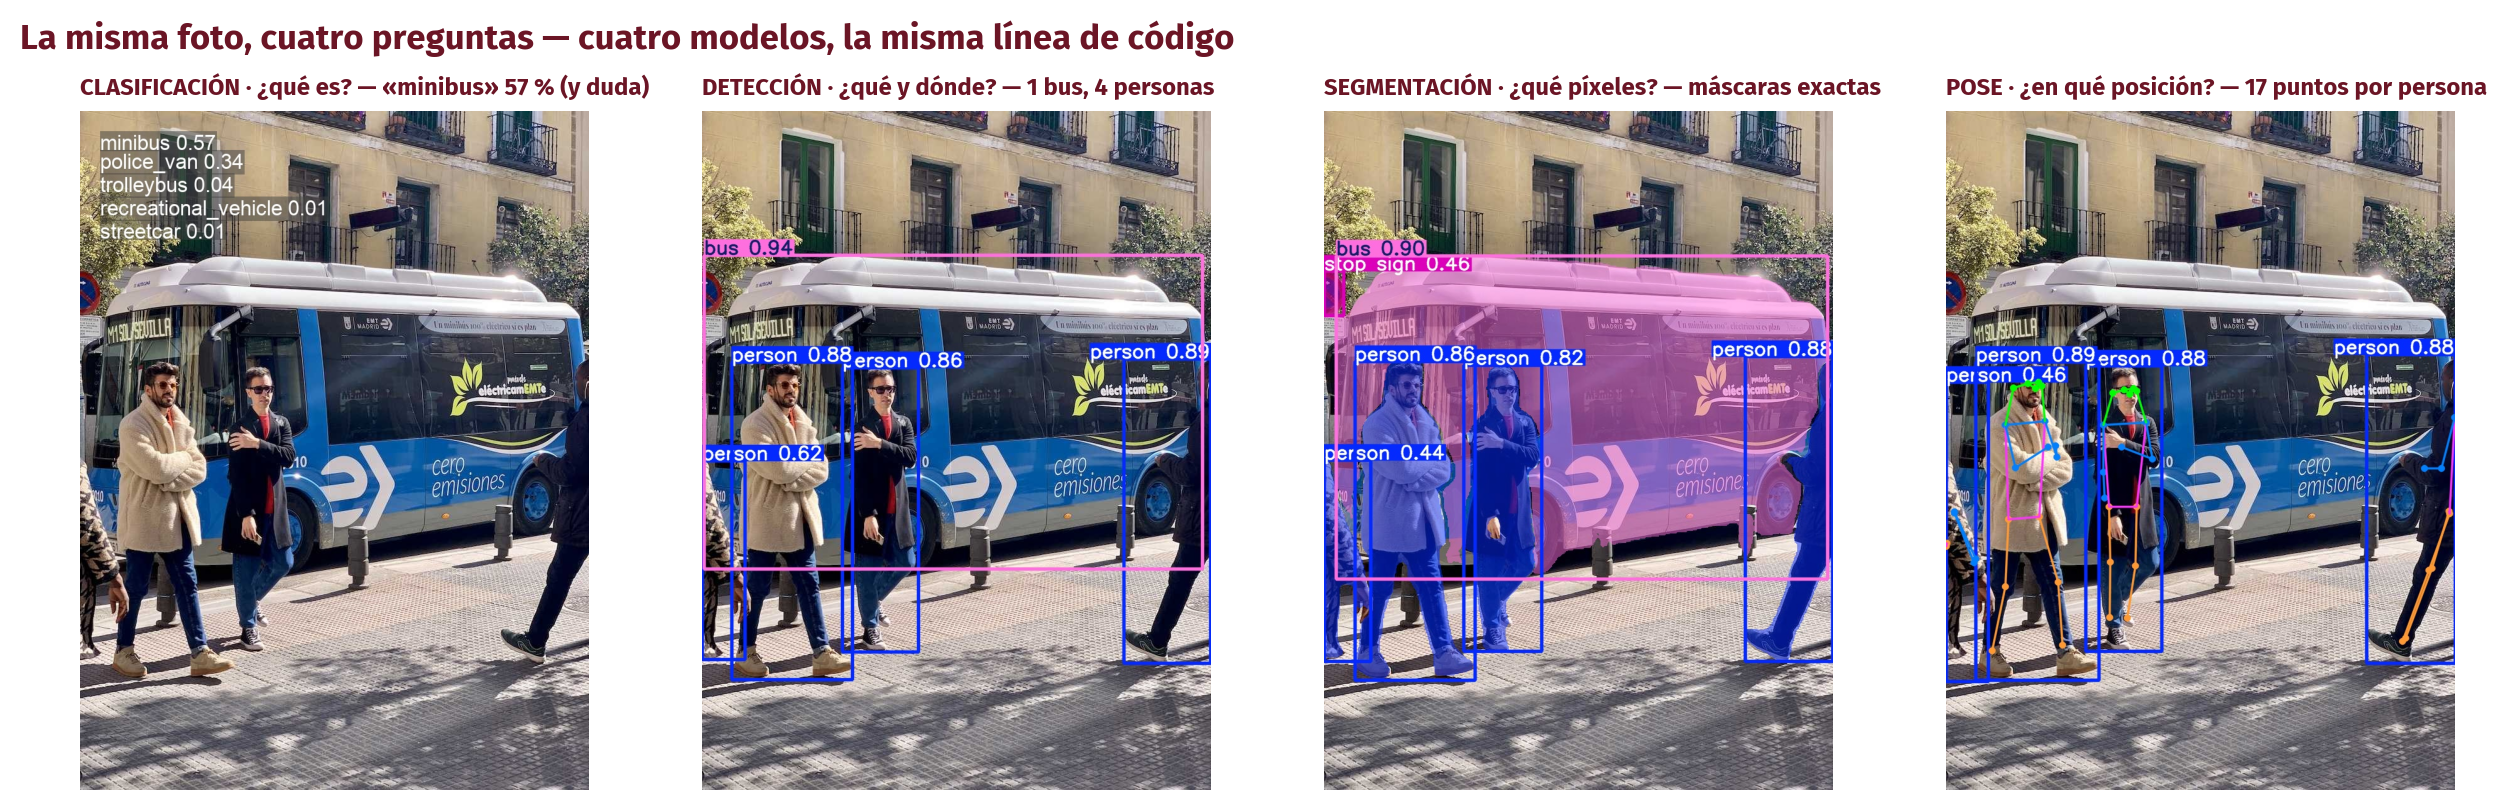
\includegraphics[width=0.99\textwidth, height=0.46\textheight, keepaspectratio]{fig_cuatro_tareas.png}\end{center}
  \vspace{2pt}
  {\footnotesize\color{textMuted}
   Corrida real, no ilustración. Los cuatro modelos de \textbf{Ultralytics}
   (\texttt{yolo11n}), cada uno con \textbf{la misma línea de código}. Vamos
   una por una.}
\end{frame}

\begin{frame}[fragile, shrink=5]{4.1 · Clasificación --- y una Lección Gratis}
  \vspace{2pt}
  \begin{minted}[fontsize=\scriptsize, breaklines]{python}
r = YOLO("yolo11n-cls.pt")("foto.jpg")[0]

for i in r.probs.top5[:3]:          # las 3 mejores apuestas
    print(r.names[i], float(r.probs.data[i]))
# minibus 0.57 | police_van 0.34 | trolleybus 0.04
  \end{minted}
  \vspace{5pt}
  {\footnotesize\color{textMuted}
   El resultado se \textbf{lee}, no solo se mira: \texttt{r.probs} trae la
   probabilidad de cada clase.}
  \vspace{5pt}
  \begin{tcolorbox}[colback=arcaGray, colframe=arcaRed, boxrule=0pt,
    leftrule=3pt, arc=3pt, left=8pt, right=8pt, top=4pt, bottom=4pt]
    {\scriptsize\color{arcaRed}\bfseries FÍJENSE: EL MODELO DUDA}\\[2pt]
    {\footnotesize\color{textMuted}
     minibus 57\,\%, police\_van 34\,\%. Una sola etiqueta para toda la
     imagen es poco cuando la imagen tiene muchas cosas --- por eso existe
     la siguiente tarea.}
  \end{tcolorbox}
\end{frame}

\begin{frame}[fragile, shrink=5]{4.2 · Detección --- el Conteo Sale de las Cajas}
  \vspace{2pt}
  \begin{minted}[fontsize=\scriptsize, breaklines]{python}
r = YOLO("yolo11n.pt")("foto.jpg")[0]

conteo = Counter(r.names[int(c)] for c in r.boxes.cls)
# {'bus': 1, 'person': 4}   confianzas: 0.94, 0.89, 0.88, ...
  \end{minted}
  \vspace{5pt}
  {\footnotesize\color{textMuted}
   \texttt{r.boxes}: una caja por objeto --- clase, confianza y coordenadas.
   Y la frase que convierte la demo en herramienta:}
  \vspace{5pt}
  \begin{tcolorbox}[colback=arcaGray, colframe=arcaDark, boxrule=0pt,
    leftrule=4pt, arc=3pt, left=10pt, right=10pt, top=6pt, bottom=6pt]
    {\footnotesize\color{arcaDark}\bfseries
     El conteo sale de \texttt{r.boxes}, no del dibujo. Una app de EPP
     filtra esas cajas («persona sin casco») --- no mira la imagen bonita.}
  \end{tcolorbox}
\end{frame}

\begin{frame}[fragile, shrink=5]{4.3 · Segmentación --- la Caja Dice Dónde; la Máscara, Cuánto}
  \vspace{2pt}
  \begin{minted}[fontsize=\scriptsize, breaklines]{python}
r = YOLO("yolo11n-seg.pt")("foto.jpg")[0]

r.masks.data.shape        # (6, 640, 480): objetos x alto x ancho
int(r.masks.data[0].sum())  # pixeles exactos del primer objeto
  \end{minted}
  \vspace{5pt}
  {\footnotesize\color{textMuted}
   La máscara permite \textbf{medir}: área de la mancha, fracción de la
   imagen, crecimiento entre dos fotos de inspección.}
  \vspace{5pt}
  \begin{tcolorbox}[colback=arcaGray, colframe=arcaDark, boxrule=0pt,
    leftrule=3pt, arc=3pt, left=8pt, right=8pt, top=4pt, bottom=4pt]
    {\scriptsize\color{textMuted}
     Detalle de la corrida real: la segmentación encontró además un
     \texttt{stop sign} que la detección no reportó --- modelos distintos,
     sensibilidades distintas. Verificar, siempre.}
  \end{tcolorbox}
\end{frame}

\begin{frame}[fragile, shrink=5]{4.4 · Pose --- Reglas de Seguridad Sobre Geometría}
  \vspace{2pt}
  \begin{minted}[fontsize=\scriptsize, breaklines]{python}
r = YOLO("yolo11n-pose.pt")("foto.jpg")[0]

len(r.keypoints)            # 4 personas
r.keypoints.data.shape[1:]  # (17, 3): articulaciones x (x, y, conf)
  \end{minted}
  \vspace{5pt}
  {\footnotesize\color{textMuted}
   17 puntos del cuerpo por persona. Con eso se responde «¿está agachado?»,
   «¿levantó los brazos?», «¿hay alguien en el suelo?» --- reglas de
   seguridad escritas sobre coordenadas.}
  \vspace{6pt}
  \begin{tcolorbox}[colback=arcaGray, colframe=codeGreen, boxrule=0pt,
    leftrule=4pt, arc=3pt, left=10pt, right=10pt, top=5pt, bottom=5pt]
    {\footnotesize\color{arcaDark}\bfseries
     Ahora con SUS fotos: suban una (panel \faFolder), cambien
     \texttt{"foto.jpg"} por la suya, y anoten \textbf{un acierto y un
     fallo}.}\\[3pt]
    {\scriptsize\color{textMuted}
     La regla de siempre: nada de instalaciones, documentos ni personas sin
     permiso.}
  \end{tcolorbox}
\end{frame}

\begin{frame}[shrink=5]{El Ojo por Código: la Pregunta Libre}
  \vspace{2pt}
  {\footnotesize\color{textMuted}
   Las cuatro tareas tienen \textbf{catálogos fijos} (80 clases, 17 puntos).
   Para la pregunta libre --- «¿cuántos llevan casco?», «¿qué marca este
   medidor?» --- se llama a un modelo \textbf{multimodal} por código.}
  \vspace{5pt}
  \begin{tcolorbox}[colback=arcaGray, colframe=arcaRed, boxrule=0pt,
    leftrule=3pt, arc=3pt, left=8pt, right=8pt, top=4pt, bottom=4pt]
    {\scriptsize\color{arcaRed}\bfseries LA LLAVE DE LA CLASE, EN TRES PASOS}\\[2pt]
    {\footnotesize\color{textMuted}
     1 · Cópienla del chat del curso. \quad 2 · Panel \faKey\ de Colab
     $\to$ \texttt{LLAVE\_CLASE}, con acceso del cuaderno. \quad 3 ·
     \textbf{Nunca} en una celda.}\\[3pt]
    {\scriptsize\color{arcaDark}\bfseries
     Al final de la clase la revocamos en vivo: una llave compartida es una
     llave quemada. Eso es gestión de secretos.}
  \end{tcolorbox}
  \vspace{5pt}
  {\scriptsize\color{textMuted}\itshape
   Plan B si la llave no corre en su cuenta: el panel de Gemini acepta
   imágenes --- misma pregunta, sin código. Pero la versión por código es la
   que se integra a una app.}
\end{frame}

\begin{frame}[fragile, shrink=5]{Tres Preguntas Sobre la Misma Foto}
  \vspace{-6pt}
  \begin{minted}[fontsize=\scriptsize, breaklines]{python}
from google.colab import userdata
from google import genai
from PIL import Image

cliente = genai.Client(api_key=userdata.get("LLAVE_CLASE"))
foto = Image.open("foto.jpg")

r = cliente.models.generate_content(
    model="gemini-2.5-flash",
    contents=[foto, "¿Cuántas personas se ven? Solo el número."])
print(r.text)
  \end{minted}
  \vspace{2pt}
  {\scriptsize\color{textMuted}
   Tres pedidos en el cuaderno: \textbf{describir}, \textbf{contar} y
   \textbf{leer} (ahí vive el OCR).}
  \vspace{2pt}
  \begin{tcolorbox}[colback=arcaGray, colframe=arcaRed, boxrule=0pt,
    leftrule=3pt, arc=3pt, left=8pt, right=8pt, top=2pt, bottom=2pt]
    {\scriptsize\color{textMuted}
     \textbf{\color{arcaRed}La advertencia al cubo:} cada foto enviada por
     esta vía \textbf{sale hacia un tercero}. Con la de la planta --- parte
     5, ya mismo.}
  \end{tcolorbox}
\end{frame}

% ═════════════════════════════════════════════════════════════════════════════
\sectionframe{5 · Los Peligros, con Nombre}{La promesa pendiente, pagada \\[6pt] \normalsize 95 -- 112 min}
% ═════════════════════════════════════════════════════════════════════════════

\begin{frame}[shrink=5]{5.1 · Lo que Se Pega, Sale de la Empresa}
  \vspace{2pt}
  {\footnotesize\color{textMuted}
   Los proveedores de estos servicios pueden \textbf{retener} lo que se les
   envía --- prompts, datos, fotos --- por meses, y \textbf{personas} pueden
   revisarlo. No es teoría: está en la letra chica de casi todos, incluido
   el Gemini de Colab (retención de hasta 18 meses, revisores humanos).}
  \vspace{6pt}
  \begin{tcolorbox}[colback=arcaGray, colframe=arcaRed, boxrule=0pt,
    leftrule=4pt, arc=3pt, left=10pt, right=10pt, top=6pt, bottom=6pt]
    {\footnotesize\color{textMuted}
    \begin{itemize}\setlength{\itemsep}{3pt}
      \item[{\color{arcaRed}\scriptsize\faLock}]
        El dato confidencial \textbf{no se pega}: producción real,
        presiones, coordenadas, nombres de pozos o clientes, fotos de
        instalaciones.
      \item[{\color{codeGreen}\scriptsize\faCheck}]
        El \textbf{esquema sí}: nombres de columnas y tipos, sin valores.
        El agente escribe el código; el código corre localmente sobre el
        dato real.
      \item[{\color{arcaRed}\scriptsize\faQuestion}]
        En la duda: seguridad de la información, \textbf{antes} --- no
        después.
    \end{itemize}}
  \end{tcolorbox}
\end{frame}

\begin{frame}[shrink=5]{5.2 · Las Llaves Son Contraseñas}
  \vspace{4pt}
  {\footnotesize\color{textMuted}
   Lo acaban de vivir: la llave fue al \textbf{Secret}, no a la celda. ¿Por
   qué tanto cuidado?}
  \vspace{6pt}
  {\footnotesize\color{textMuted}
  \begin{itemize}\setlength{\itemsep}{5pt}
    \item[{\color{arcaRed}\scriptsize\faArrowRight}]
      Un cuaderno \textbf{se comparte}, se sube a un repositorio, se
      proyecta en una reunión. Una llave pegada en una celda queda expuesta
      en todos esos lugares a la vez.
    \item[{\color{arcaRed}\scriptsize\faArrowRight}]
      Una llave expuesta es \textbf{plata}: alguien consume el servicio a
      nombre de ustedes --- o algo peor con lo que la llave alcance.
    \item[{\color{codeGreen}\scriptsize\faArrowRight}]
      Por eso: secrets, \textbf{rotación}, y revocar cuando se compartió de
      más.
  \end{itemize}}
  \vspace{7pt}
  \begin{tcolorbox}[colback=arcaGray, colframe=arcaDark, boxrule=0pt,
    leftrule=4pt, arc=3pt, left=10pt, right=10pt, top=6pt, bottom=6pt]
    {\footnotesize\color{arcaDark}\bfseries
     La nuestra muere hoy, delante de ustedes. Una llave compartida es una
     llave quemada --- y quemarla a tiempo es el trabajo bien hecho.}
  \end{tcolorbox}
\end{frame}

\begin{frame}[shrink=5]{5.3 · Las Librerías Alucinadas}
  \vspace{2pt}
  {\scriptsize\color{textMuted}
   Un agente puede recomendar, con total confianza, una librería \textbf{que
   no existe}. Y hay algo peor: que \emph{sí} exista --- porque alguien la
   registró con el nombre que los agentes suelen inventar, cargada de código
   malicioso (\emph{typosquatting} y \emph{slopsquatting}: registrar el
   error esperable).}
  \vspace{2pt}
  \begin{tcolorbox}[colback=arcaGray, colframe=arcaDark, boxrule=0pt,
    leftrule=4pt, arc=3pt, left=10pt, right=10pt, top=4pt, bottom=4pt]
    {\scriptsize\color{arcaDark}\bfseries LA DEFENSA: 30 SEGUNDOS ANTES DE CADA pip install}\\[2pt]
    {\scriptsize\color{textMuted}
    \begin{itemize}\setlength{\itemsep}{2pt}
      \item ¿Existe en PyPI, con página y documentación reales?
      \item ¿Cuántas descargas, desde cuándo, quién la mantiene?
      \item ¿De verdad hace falta? Si el agente propone una librería exótica
            para algo que pandas ya hace --- desconfíen.
    \end{itemize}}
  \end{tcolorbox}
  \vspace{2pt}
  {\scriptsize\color{arcaDark}\itshape
   Las de este curso --- pandas, scikit-learn, keras, gradio, ultralytics,
   shap --- son masivas y auditadas. La regla es para la que no conocen.}
\end{frame}

\begin{frame}[shrink=5]{5.4 · El Peor de Todos: Código que Corre y Está Mal}
  \vspace{2pt}
  {\scriptsize\color{textMuted}
   No lanza error. Produce un número. El número es basura. Lo vieron
   \textbf{tres veces} en este módulo:}
  \vspace{2pt}
  {\scriptsize\color{textMuted}
  \begin{itemize}\setlength{\itemsep}{2pt}
    \item[{\color{arcaRed}\scriptsize\faTimes}]
      Las propinas en efectivo: \textbf{cero} que era ausencia (C1)
    \item[{\color{arcaRed}\scriptsize\faTimes}]
      La columna \texttt{alive}: accuracy \textbf{1.000} que era trampa (C3)
    \item[{\color{arcaRed}\scriptsize\faTimes}]
      El tasador: \textbf{USD 397} por una piedra de 0 mm (C2)
  \end{itemize}}
  \vspace{2pt}
  \begin{tcolorbox}[colback=arcaGray, colframe=codeGreen, boxrule=0pt,
    leftrule=4pt, arc=3pt, left=10pt, right=10pt, top=4pt, bottom=4pt]
    {\scriptsize\color{codeGreen}\bfseries LA DEFENSA ES LA DE LA CLASE 1 --- Y NO CADUCA}\\[2pt]
    {\scriptsize\color{textMuted}
     1 · ¿Cuántas filas entraron y cuántas salieron? \quad
     2 · ¿Ceros, vacíos o números perfectos? \\
     3 · ¿Tiene sentido físico o de negocio? \quad
     4 · ¿Qué decisión se toma con esto, y qué pasa si está mal?}
  \end{tcolorbox}
  \vspace{2pt}
  {\scriptsize\color{arcaDark}\bfseries\itshape
   Cuatro preguntas, dos minutos, cero programación. Es la herramienta más
   barata y más rentable de todo el diplomado.}
\end{frame}

% ═════════════════════════════════════════════════════════════════════════════
\sectionframe{6 · Cierre}{}
% ═════════════════════════════════════════════════════════════════════════════

\begin{frame}[shrink=5]{Su Entrega del Jueves}
  \vspace{2pt}
  {\footnotesize\color{textMuted}
   Equipos de hasta 3. El cuaderno del Titanic es la plantilla. Se entrega:}
  \vspace{5pt}
  {\footnotesize\color{textMuted}
  \begin{itemize}\setlength{\itemsep}{4pt}
    \item[{\color{codeGreen}\scriptsize\faCheck}]
      El \textbf{cuaderno} con el flujo completo: EDA $\to$ limpieza con
      decisiones escritas $\to$ comparación de modelos $\to$ examen
      reservado $\to$ explicabilidad
    \item[{\color{codeGreen}\scriptsize\faCheck}]
      La \textbf{app} con su link funcionando
    \item[{\color{codeGreen}\scriptsize\faCheck}]
      Los \textbf{prompts} que usaron
    \item[{\color{codeGreen}\scriptsize\faCheck}]
      \textbf{Un error del agente que ustedes cazaron}, y cómo lo detectaron
    \item[{\color{codeGreen}\scriptsize\faCheck}]
      Qué \textbf{decisión} habilita la herramienta, y para quién
  \end{itemize}}
  \vspace{6pt}
  \begin{tcolorbox}[colback=arcaGray, colframe=arcaDark, boxrule=0pt,
    leftrule=3pt, arc=3pt, left=8pt, right=8pt, top=4pt, bottom=4pt]
    {\scriptsize\color{arcaDark}\bfseries
     El error cazado vale tanto como la app: demuestra que dirigieron, no
     que obedecieron.}
  \end{tcolorbox}
\end{frame}

\begin{frame}[shrink=5]{El Módulo, en Cuatro Clases}
  \vspace{2pt}
  \begin{center}
  {\footnotesize
  \begin{tabular}{cl}
    \toprule
    \textbf{Clase} & \textbf{Lo que quedó} \\
    \midrule
    1 & Dirigir un agente: los cuatro fundamentos, y verificar siempre \\[2pt]
    2 & Un modelo servido: certificar, entrenar, examinar, blindar \\[2pt]
    3 & El flujo profesional (GridSearch, SHAP) --- y su primera red \\[2pt]
    4 & Las máquinas que ven, el ojo por código, y los peligros \\
    \bottomrule
  \end{tabular}}
  \end{center}
  \vspace{2pt}
  \begin{tcolorbox}[colback=arcaGray, colframe=arcaRed, boxrule=0pt, leftrule=4pt,
    arc=3pt, left=10pt, right=10pt, top=4pt, bottom=4pt]
    {\large\color{arcaDark}\bfseries
     El agente escribe. Ustedes responden.}\\[2pt]
    {\scriptsize\color{textMuted}
     Escribir se volvió barato. El criterio para especificar bien, verificar
     siempre y desconfiar de lo perfecto --- eso es lo que ustedes ponen, y
     vale más ahora que hace tres años.}
  \end{tcolorbox}
\end{frame}

\begin{frame}[shrink=8]{Datos y Referencias}
  \vspace{4pt}
  {\footnotesize\color{textMuted}
  \begin{itemize}\setlength{\itemsep}{5pt}
    \item[{\color{arcaRed}\scriptsize\faDatabase}]
      \textbf{Fashion-MNIST}: Xiao, Rasul \& Vollgraf (Zalando Research,
      2017), vía \texttt{keras.datasets}. \textbf{Foto de prueba}: assets de
      Ultralytics.
    \item[{\color{arcaRed}\scriptsize\faBook}]
      \textbf{YOLO}: Redmon et al.\ (2016); implementación
      \textbf{Ultralytics} (yolo11n: cls/det/seg/pose). \textbf{AlexNet}:
      Krizhevsky, Sutskever \& Hinton (2012). \textbf{Gemini API}: SDK
      \texttt{google-genai}.
    \item[{\color{arcaRed}\scriptsize\faFileCode}]
      La solución de referencia y las imágenes anotadas salen de
      \texttt{figuras.py} (semilla fija; corridas reales, no ilustraciones).
      La solución en vivo se corre con Keras y varía en decimales.
  \end{itemize}}
  \vspace{7pt}
  {\scriptsize\color{arcaDark}\itshape
   Como siempre: corren los scripts y tiene que dar lo mismo. Si no da, es
   un error nuestro y queremos saberlo.}
\end{frame}

% ── GRACIAS ──────────────────────────────────────────────────────────────────
\begingroup
\setbeamertemplate{headline}{}
\setbeamertemplate{footline}{}
\setbeamertemplate{navigation symbols}{}
\begin{frame}[plain, noframenumbering]
  \begin{tikzpicture}[remember picture, overlay]
    \fill[arcaDark] (current page.south west) rectangle (current page.north east);
    \node[anchor=center, text=white, font=\Huge\bfseries]
      at ([yshift=1.5cm]current page.center) {¡Gracias!};
    \node[anchor=center, text=white!80, font=\large, text width=10cm, align=center]
      at ([yshift=0.2cm]current page.center)
      {Carlos Enrique Mosquera Trujillo};
    \node[anchor=center, text=white!60, font=\normalsize, text width=10cm, align=center]
      at ([yshift=-0.6cm]current page.center)
      {\faEnvelope\hspace{6pt}cmosquerat@unal.edu.co};
    \node[anchor=center, text=white!60, font=\normalsize, text width=11cm, align=center]
      at ([yshift=-1.3cm]current page.center)
      {Machine Learning for Petroleum Engineers Using Python};
    \node[anchor=center, text=white!40, font=\small]
      at ([yshift=-2.0cm]current page.center)
      {Módulo 7 · Clase 4 \quad$\cdot$\quad SLB Ecuador \quad$\cdot$\quad UDLA \quad$\cdot$\quad 2026};
  \end{tikzpicture}
\end{frame}
\endgroup

\end{document}
